\documentclass[aspectratio=169,10pt]{beamer}

% ------------------------------------------------
% PACKAGES AND CONFIG

\usepackage[T1]{fontenc}
\usepackage[utf8]{inputenc}
\usepackage{FiraSans,FiraMono} % \usepackage{tgheros}

\usepackage[french,english]{babel}
\usepackage{csquotes}

\usepackage{booktabs}
\usepackage{transparent}
\usepackage[dvipsnames,table]{xcolor}
\usepackage[most]{tcolorbox}
\usepackage{tabularx}
\usepackage{multirow}
\usepackage[export]{adjustbox}
\usepackage[symbol]{footmisc}

\usepackage{biblatex}
\renewcommand\bibfont{\small}
\DeclareBibliographyCategory{standout}
\AtDataInput{%
  \iffieldequalstr{usera}{standout}%
  {\addtocategory{standout}{\thefield{entrykey}}}%
  {}%
}{}
\DeclareFieldFormat{labelnumber}{%
  \ifcategory{standout}{\mkbibbold{\textexample{#1}}}{#1}%
}
\addbibresource{lavaur.bib}
\addbibresource{references.bib}

\usepackage[mode=buildnew]{standalone}
\renewcommand<>{\includestandalone}[2][]{%
  \only#3{\beameroriginal{\includestandalone}[#1]{#2}}%
}

\usepackage{caption}
\captionsetup{font=small}

\usepackage[acronym]{glossaries}
\glsdisablehyper
\loadglsentries{glossary}

\usepackage{tikz}
\usetikzlibrary{calc,positioning,trees}

\usepackage[]{minted}

\usepackage{useful}
% ------------------------------------------------
% THEME
\usetheme[
  progressbar=foot,
  titleformat frame=smallcaps,
  sectionpage=none,
  subsectionpage=none,
  %titlepage style=fancy,
]{moloch}

% ----------------------------------------
% Colors and theming
\definecolor{sntred}{HTML}{d22739}
\definecolor{sntpurple}{HTML}{64267f}
\definecolor{sntblue}{HTML}{0e81c2}
\setbeamercolor{alerted text}{fg=sntblue}
\setbeamercolor{example text}{fg=sntpurple}

\setbeamercolor{normal text}{bg=white}
\setbeamercolor{frametitle}{fg=white}
\setbeamertemplate{page number in head/foot}[appendixframenumber]
\setbeamertemplate{section}[sections numbered]

% Item indent
\setlength{\leftmargini}{1.5em}

\setbeamertemplate{footline}{%
  \begin{beamercolorbox}[
      leftskip=4pt,%
      rightskip=4pt,%
      wd=\textwidth,%
    ]{footline}%
    \usebeamercolor[fg]{page number in head/foot}%
    \usebeamerfont{page number in head/foot}%
    \usebeamertemplate*{frame footer}%
    \hfill%
    \usebeamertemplate*{page number in head/foot}%
    \vskip2pt%
    \usebeamertemplate*{progress bar in head/foot}%
  \end{beamercolorbox}%
}

\makeatletter
\def\maketitle{%
  \ifbeamer@inframe
  \titlepage
  \else
  \begingroup
  \renewcommand\footnoterule{}%
  \usebackgroundtemplate{
\includegraphics[width=\paperwidth]{assets/backgrounds/background-normal}}%
  \setbeamercolor{normal text}{fg=white}%
  \frame[plain,noframenumbering]{\titlepage}
  \endgroup
  \fi
}
\setbeamertemplate{title page}{
  \null%
  \vspace{0pt plus 1.618fil}%
  \vfil%
  
\includegraphics[width=0.1\paperwidth]{assets/logos/SnT_white}\\%
  \vspace{1ex}%
  \ifx\inserttitle\@empty\else\usebeamertemplate*{title}\fi
  \ifx\insertsubtitle\@empty\else\usebeamertemplate*{subtitle}\fi
  \expandafter\ifblank\expandafter{\beamer@andstripped}{}{%
    \vspace{2ex}%
    \usebeamertemplate*{author}%
  }
  \ifx\insertinstitute\@empty\else\usebeamertemplate*{institute}\fi
  \ifx\insertdate\@empty\else\vspace{.5ex}\usebeamertemplate*{date}\fi
  \vspace{0pt plus 1fil}%
  \null
  \begin{tikzpicture}[remember picture,overlay,shift={(current page.south east)}]
    \node[anchor=south east] (snt-ul) {
\includegraphics[width=0.22\paperwidth]{assets/logos/SnT_UL_white}};
    \node[anchor=south east] at (snt-ul.south west) {%
      \ifx\inserttitlegraphic\@empty\else\usebeamertemplate*{title graphic}\fi
    };
  \end{tikzpicture}
}
\makeatother

\AtBeginEnvironment{frame}{\setcounter{footnote}{0}}


\hypersetup{
  colorlinks,
  citecolor=sntblue,
  linkcolor=.,
}
% ------------------------------------------------
% MACROS

\definecolor{contrib/eiffel}{HTML}{FFE599}
\definecolor{contrib/radar}{HTML}{F19C99}
\definecolor{contrib/feditn}{HTML}{B9E0A5}
\definecolor{contrib/slr}{HTML}{C4D1E3}
\definecolor{contrib/waterllmarks}{HTML}{ac9cc1}
\definecolor{contrib/logic}{HTML}{B1DDF0}
\definecolor{contrib/flb}{HTML}{F8CECC}
\definecolor{contrib/rag}{HTML}{FFCE99}

\newcommand\slr{\circled{contrib/slr}{S}\xspace}
\newcommand\eiffel{\circled{contrib/eiffel}{E}\xspace}
\newcommand\radar{\circled{contrib/radar}{R}\xspace}
\newcommand\feditn{\circled{contrib/feditn}{F}\xspace}
\newcommand\waterllmarks{\circled{contrib/waterllmarks}{W}\xspace}
\newcommand\logic{\circled{contrib/logic}{L}\xspace}
\newcommand\flb{\circled{contrib/flb}{G}\xspace}
\newcommand\rag{\circled{contrib/rag}{A}\xspace}

% -----------------------------------------------
% DOCUMENT

\title{Confidential Collaboration for Reliable Detection in Distributed Systems}
\author{Léo Lavaur}
\institute{
  Interdisciplinary Centre for Security, Reliability and Trust (SnT)\\
Université du Luxembourg}
\date{\footnotesize June 10\textsuperscript{th}\kern-0.3em, 2026 $\cdot$
\foreignlanguage{french}{Journées Nationales du GDR SSI, Lille}}

\begin{document}

\maketitle

\section*{Introduction}

\begin{frame}{\ttfamily ./whoami}
  \begin{columns}
    \column{0.75\textwidth}
    \begin{description}
        \setlength{\itemsep}{2ex}
      \item[2024--\textit{now}\hfill] Postdoc, University of Luxembourg, SnT, Luxembourg\\
        {\small\color{gray}
          \alert{Security} and \alert{monitoring} of locally distributed systems.\\
        With \textexample{Jérôme François}, academic (COCTEL, FNR) and industrial (PAIGE, Thales Luxembourg) projects.}
      \item[2020--2024\hfill] PhD, IMT Atlantique, IRISA/SOTERN, Rennes\\
        {\small\color{gray} "Improving \alert{intrusion detection} in distributed systems with \alert{federated learning}"\\
          Supervised by \textexample{Yann Busnel}, co-supervised by \textexample{Fabien Autrel} and \textexample{Marc-Olivier Pahl}, industrial funding (Chair CyberCNI).\\
        \textbf{GDR RSD PhD Thesis Award, 2025}.}
      \item[2017--2020\hfill] Eng. Degree in Information Security, ENSIBS, Vannes\\
        {\small\color{gray} Part-time employee at Orange Cyberdefense, Rennes, \alert{application security} and DevSecOps.}
    \end{description}

    \column{0.30\textwidth}
    \centering
    \includegraphics[width=.9\linewidth]{figures/lavaur_snt.png}
    \vspace{1em}

    Intrusion Detection\\
    Federated Learning\\
    Security of AI Systems\\
    Network/System Security\\

  \end{columns}

  \begin{minipage}{0.85\textwidth}
  \end{minipage}
\end{frame}

\begin{frame}[t]{Intrusion Detection in Organizations}

  \begin{columns}
    \column{0.55\textwidth}
    \begin{block}{Intrusion detection system (IDS)}
      Automated tool for identifying \alert{malicious} activity
    \end{block}

    \onslide<3->{%
      \begin{block}{Solved\only<4>{{\usebeamercolor{alerted text}\color{fg}\footnotemark}} thanks to machine learning!}
        99\% accuracy on public benchmarks
    \end{block}}

    \column{0.45\textwidth}
    \centering%
    \includegraphics<1>[width=1.1\textwidth,center]{figures/intro/ids-1.pdf}%
    \includegraphics<2>[width=1.1\textwidth,center]{figures/intro/ids-2.pdf}%
    \includegraphics<3->[width=1.1\textwidth,center]{figures/intro/ids-3.pdf}%
  \end{columns}

  \only<4>{\footnotetext{Assuming high-quality datasets that are representative of real-world scenarios\dots}}
\end{frame}

% \begin{frame}[t]{Collaboration and Federated Learning}
%   \setbeamercolor{itemize item}{fg=example text.fg}\vspace{-1em}
%   \vspace{1em}
%   \begin{columns}
%     \column{0.5\textwidth}
%     \begin{itemize}[<+->]
%         \setlength{\itemsep}{1ex}
%       \item Similar tasks in numerous organizations
%       \item Towards collaborative approaches?
%       \item Data too sensitive to be shared
%       \item Solution: \alert{federated learning} (FL)
%     \end{itemize}

%     \column{0.5\textwidth}
%     \centering
%     \foreach \i in {1,...,3} {\includegraphics<\i>[width=1.1\textwidth,center]{figures/intro/cids-\i.pdf}}%
%     \includegraphics<4->[width=1.1\textwidth,center]{figures/intro/fids.pdf}%

%   \end{columns}

%   \onslide
%   \begin{center}
%     {\large\bfseries Can \alert{FL} serve as a \alert{collaboration} tool for intrusion detection?}
%   \end{center}
% \end{frame}

\begin{frame}[t]{A Distributed Problem}
  \begin{columns}
    \column{0.5\textwidth}
    \begin{block}{Similar tasks in numerous organizations}
      Different attacks and devices but same challenge
    \end{block}

    \onslide<2->{%
      \begin{block}{Incentives to collaborate}
        \begin{itemize}
          \item common interest (\eg, inter-SOCs\only<2>{\footnotemark})
          \item national agencies (\eg, NIST, ANSSI)
          \item regulation (\eg, private-public information sharing in NIS2)
        \end{itemize}
    \end{block}}

    \column{0.5\textwidth}
    \centering
    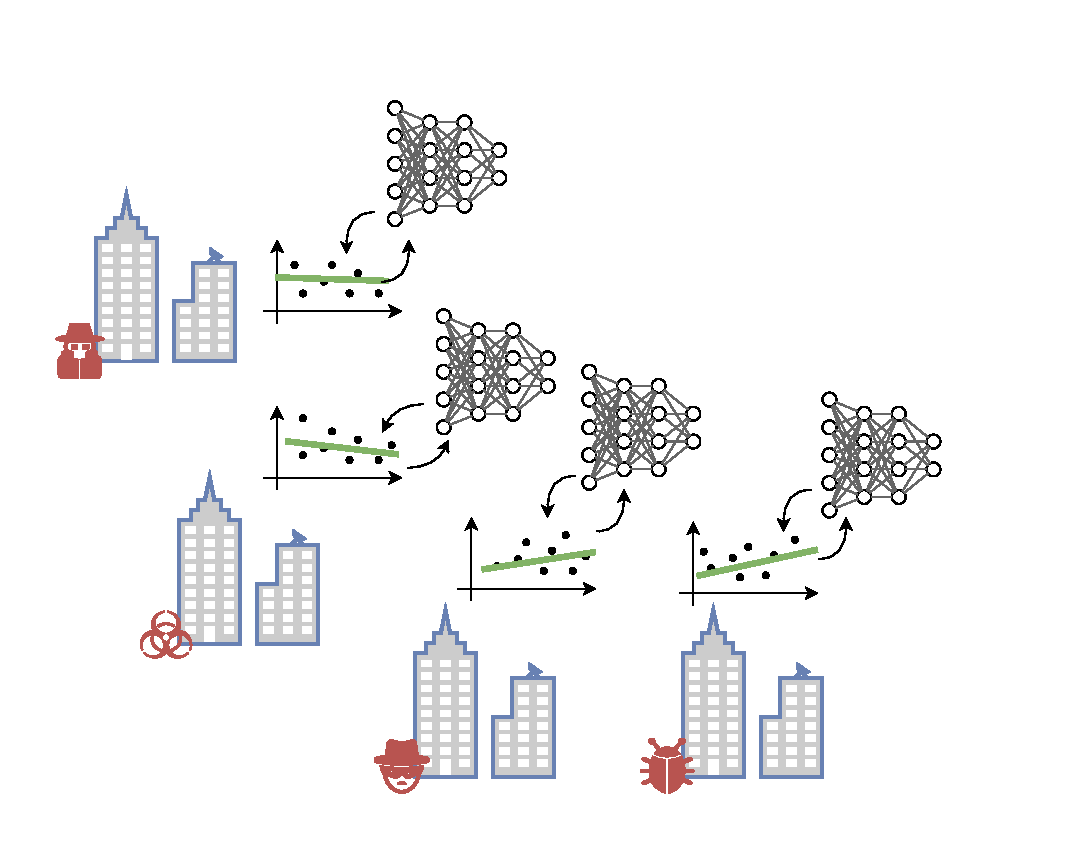
\includegraphics[width=1.1\textwidth,center]{figures/intro/cids-1.pdf}%
  \end{columns}

  \only<2->{\footnotetext{Security Operations Centers.}}
\end{frame}

\begin{frame}[t]{Collaborative Learning}
  \begin{columns}
    \column{0.5\textwidth}

    \textbf{Let's pool our data!}\onslide<2->{
      \textbf{Although\dots}

      \begin{itemize}
        \item Privacy concerns.
        \item Lack of trust in the data holder.
        \item Lack of trust in the learning process.
        \item \dots
    \end{itemize}}

    \column{0.5\textwidth}
    \centering
    \includegraphics<1>[width=1.1\textwidth,center]{figures/intro/cids-2.pdf}%
    \includegraphics<2->[width=1.1\textwidth,center]{figures/intro/cids-3.pdf}%
  \end{columns}
\end{frame}

\begin{frame}[t]{Federated Learning}
  \begin{columns}
    \column{0.5\textwidth}
    \textbf{The solution: \alert{Federated Learning} (FL)}~\autocite{mcmahan_Communicationefficientlearningdeep_2017}
    \begin{itemize}
      \item Clients train a common model without sharing data
      \item Only model updates are shared with a central server
      \item More privacy-friendly
    \end{itemize}
    \column{0.5\textwidth}
    \centering
    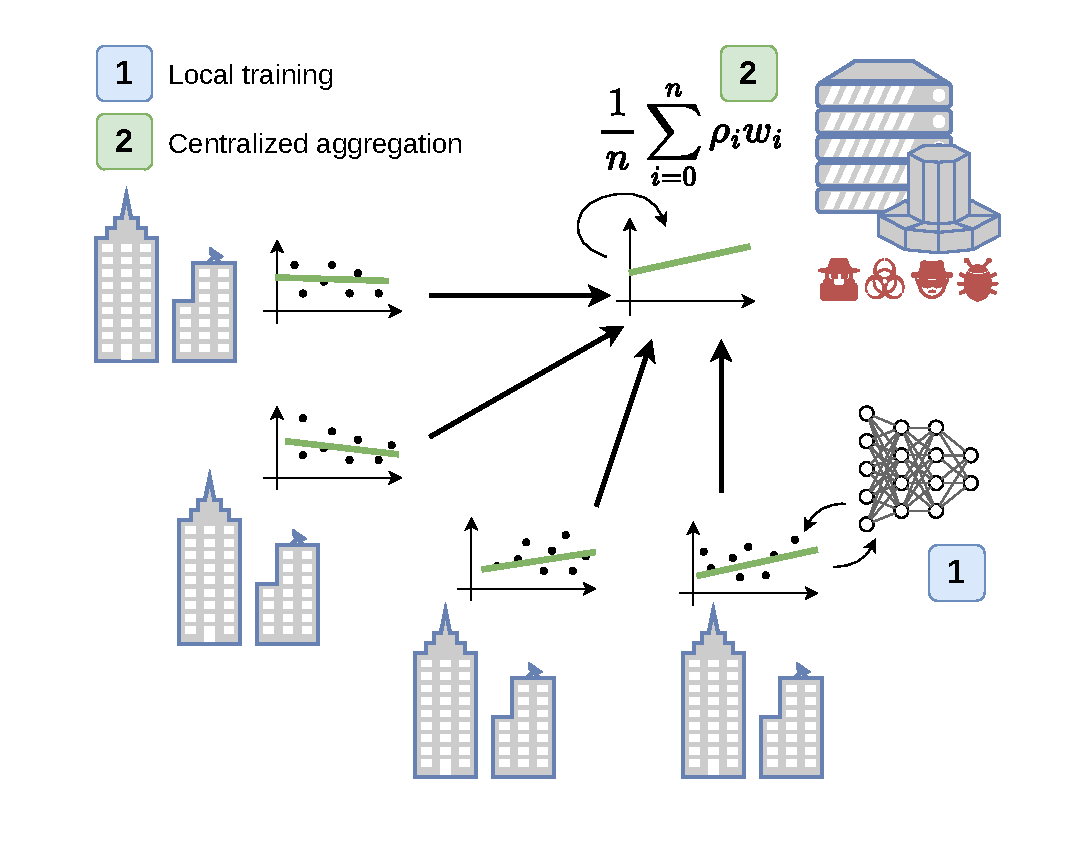
\includegraphics[width=1.1\textwidth,center]{figures/intro/fids.pdf}%
  \end{columns}
  \pause
  \only<1>{\footcite*{mcmahan_Communicationefficientlearningdeep_2017}}
  \only<2->{
    \begin{center}
      {\large\bfseries Can \alert{FL} serve as a \alert{collaboration} tool for intrusion detection?}
    \end{center}
  }
\end{frame}
\input{sections/20_phd}
\section{\texorpdfstring{\logic Neural-symbolic Integration for Attack Detection}{Neural-symbolic Integration for Attack Detection}}

% Legend item style for metro map overlay
\tikzset{legenditem/.style={
    %fill=white,
    %draw=gray!30,
    %rounded corners=2pt,
    inner ysep=1pt,
    inner xsep=3pt,
    %outer sep=0pt,
    minimum width=12.5em,
    text width=12.5em,
    font=\scriptsize,
    %align=left,
    anchor=north west
}}
\tikzset{largeitem/.style={
    legenditem,
    minimum width=20em,
    text width=20em,
}}
\tikzset{citeitem/.style={
    inner sep=3pt,
    text width=0.75\textwidth,
    font=\scriptsize,
    yshift=.2ex,
}}

\begin{frame}%{Contributions overview -- PhD}

  \alt<2->{\frametitle{Contributions overview -- Postdoc}}{\frametitle{Contributions overview -- PhD}}

  \begin{tikzpicture}[remember picture, overlay, shift={(current page.south west)}, x=\paperwidth, y=\paperheight]%
    \node[anchor=south, yshift=-5pt] at (current page.south) {
      \foreach \i in {4,5,5,6,7,8} {%
        \includegraphics<+>[height=.95\textheight]{figures/metro/\i.pdf}%
      }%
      \includegraphics<+>[height=.95\textheight]{figures/metro/8-transparent.pdf}%
    };

    \alt<1-5>{
      \node[legenditem] (legend-0-0) at (0.02,0.3) {\hspace{1.4em}\textbf{CONTRIBUTIONS}};
      \node[legenditem] (legend-0-1) at (legend-0-0.south west) {\slr \texttt{Survey (SLR)}~\autocite{lavaur_tnsm_2022,lavaur_cesar_2022}};
      \node[legenditem] (legend-0-2) at (legend-0-1.south west) {\eiffel \texttt{Assessment \& eiffel}~\autocite{lavaur_icdcs_demo_2024,lavaur_ares_bass_2024,lavaur_cose_2025}};
      \node[legenditem] (legend-0-3) at (legend-0-2.south west) {\radar \texttt{RADAR}~\autocite{lavaur_radar_2024,lavaur_algotel_2025}};
      \node[legenditem] (legend-0-4) at (legend-0-3.south west) {\feditn \texttt{FedITN}~\autocite{lavaur_anubis_2025}};
    }{
      \node[legenditem, opacity=0.3] (legend-0-0) at (0.02,0.3) {\hspace{1.4em}\textbf{CONTRIBUTIONS}};
      \node[legenditem,opacity=0.3] (legend-0-1) at (legend-0-0.south west) {\slr \texttt{Survey (SLR)}~\autocite{lavaur_tnsm_2022,lavaur_cesar_2022}};
      \node[legenditem,opacity=0.3] (legend-0-2) at (legend-0-1.south west) {\eiffel \texttt{Assessment \& eiffel}~\autocite{lavaur_icdcs_demo_2024,lavaur_ares_bass_2024,lavaur_cose_2025}};
      \node[legenditem,opacity=0.3] (legend-0-3) at (legend-0-2.south west) {\radar \texttt{RADAR}~\autocite{lavaur_radar_2024,lavaur_algotel_2025}};
      \node[legenditem,opacity=0.3] (legend-0-4) at (legend-0-3.south west) {\feditn \texttt{FedITN}~\autocite{lavaur_anubis_2025}};
    }

    \only<2-5>{
      \node[legenditem,yshift=-.3ex] (legend-0-5) at (legend-0-4.south west) {\hspace{1.4em}\textbf{ONGOING WORK}};
      \node[largeitem] (legend-0-6) at (legend-0-5.south west) {\flb \texttt{Gossip learning for WSNs\textsuperscript{$\ddagger$}}};
    }
    \only<6>{
      \node[legenditem,yshift=-.3ex,opacity=0.3] (legend-0-5) at (legend-0-4.south west) {\hspace{1.4em}\textbf{ONGOING WORK}};
      \node[largeitem,opacity=0.3] (legend-0-6) at (legend-0-5.south west) {\flb \texttt{Gossip learning for WSNs\textsuperscript{$\ddagger$}}};
    }
    \only<2>{
      \node[citeitem, anchor=south east] at (current page.south east) {\textsuperscript{$\ddagger$}~Collab. with \textexample{H. Rivano} (INSA Lyon; Citi/Agora). One submission.};
    }
    \only<3>{
      \node[fill=white, opacity=0.5, minimum width=\paperwidth, minimum height=\paperheight] at (current page.center) {};
      \node[anchor=center, draw=gray, rounded corners=3pt, inner sep = 10pt, fill=white] at (current page.center) {
        \begin{minipage}{.8\paperwidth}
          \textbf{COCTEL: Causality-Oriented Cybersecurity TELemetry}~\logic~\waterllmarks
          \begin{itemize}
            \item \alert{\bfseries Goal:} how to extract and represent relationships between distributed events, allowing forward and backward reasoning about them.
            \item Academic project, FNR funding (Luxembourgish national research fund), PI: Jérôme François (SnT).
          \end{itemize}
      \end{minipage}};
      \node[anchor=south east, xshift=-1em, yshift=1em] at (current page.south east) {%
        \raisebox{-0.5\height}{
\includegraphics[height=1.2cm]{assets/logos/SnT_UL_colour.pdf}}%
        \hspace{-.5em}\raisebox{-0.5\height}{
\includegraphics[height=1cm]{assets/logos/FNR_LOGO_BIG.pdf}}%
      };
    }

    \only<4-6>{
      \node[legenditem,anchor=north west] (legend-1-1) at (legend-0-1.north east) {\waterllmarks \texttt{WaterLLMarks}~\autocite{lavaur_waterllmarks_2025}};
    }
    \only<4>{
      \node[citeitem, anchor=south east] at (current page.south east) {\smallfullcite{lavaur_waterllmarks_2025}. Demo track ICDCS.};
    }
    \only<7->{
      \node[legenditem,opacity=0.3,anchor=north west] (legend-1-1) at (legend-0-1.north east) {\waterllmarks \texttt{WaterLLMarks}~\autocite{lavaur_waterllmarks_2025}};
    }

    \only<5-6>{
      \node[largeitem] (legend-1-2) at (legend-1-1.south west) {\rag \texttt{Semantic access control for RAG}~\autocite{thuillier_aiml_2026}};
    }
    \only<5>{
      \node[citeitem, anchor=south east] at (current page.south east) {\smallfullcite{thuillier_aiml_2026}};
    }
    \only<7->{
      \node[largeitem,opacity=0.3] (legend-1-2) at (legend-1-1.south west) {\rag \texttt{Semantic access control for RAG}~\autocite{thuillier_aiml_2026}};
    }

    \only<6->{
      \node[largeitem] (legend-1-3) at (legend-1-2.south west) {\logic \texttt{Logic and neural-symbolic integration}~\autocite{anser_fmano_2026}};
    }
    \only<6>{
      \node[citeitem, anchor=south east] at (current page.south east) {\smallfullcite{anser_fmano_2026}};
    }

  \end{tikzpicture}%
\end{frame}

%  1. Définitions/Context : raisonnement symbolique, intégration neuro symbolique
% - comp type 1/2
% - interpretability and determinism when needed
\begin{frame}[t]{Definitions}
  \begin{block}{Symbolic reasoning}
    Represents knowledge as explicit symbols (\alert{facts}) and provides \alert{rules} to derive new knowledge or make decisions.
    \pause
    Example of rule in First-Order Logic (FOL):
    \begin{equation*}
      \forall p,f: \text{IsShellProcess}(p) \land \text{Accesses}(p,f) \land \text{IsSensitiveFile}(f) \rightarrow \text{IsSuspicious}(p).
    \end{equation*}
  \end{block}

  \pause
  \begin{block}{Neural-symbolic integration}
    Combines symbolic reasoning (interpretability, explicit knowledge representation) with neural networks (learning from data, handling uncertainty). \Eg, DeepProbLog~\footcite{manhaeve_DeepProbLogNeuralProbabilistic_2018}, Scallop~\footcite{li_ScallopLanguageNeurosymbolic_2023}.
  \end{block}
\end{frame}

% 2. It all starts from a dataset...
% - casino limit
% - our goal, extract relationships between attacks
\begin{frame}{It all starts from a dataset\dots}
  \begin{columns}
    \column{0.5\textwidth}

    \textbf{The CasinoLimit dataset}~\autocite{kilian_CasinoLimitOffensiveDataset_2025}
    \begin{itemize}
      \item Controlled CTF exercise played by 114 participants, each on an isolated but identical instance.
      \item A defined 8-step scenario labeled with MITRE ATT\&CK techniques.
        \pause
      \item \alert{Our goal:} extract the scenario from the data, using classification and domain knowledge.
    \end{itemize}

    \column{0.5\textwidth}
    \vspace{-.5em}
    \centering
    \only<3>{\vspace{-2em}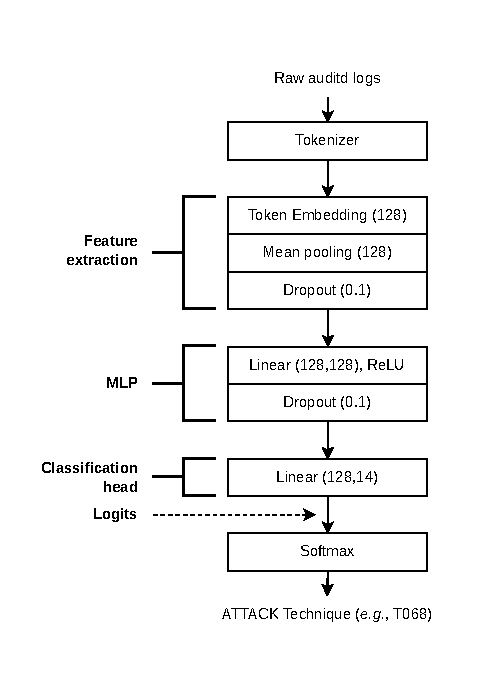
\includegraphics[width=.75\textwidth]{figures/postdoc/nesy/mlp.drawio.pdf}}%
    \includegraphics<4>[width=1.05\textwidth,center]{figures/postdoc/nesy/confmat}%
    \vfill
  \end{columns}
  \footcite*{kilian_CasinoLimitOffensiveDataset_2025}
\end{frame}

% 4. Adding contexte (arch neuro sym with animations)
% - usually in ml we do window (mention lstm/transformer)
% - logit rerank at inference

\begin{frame}{Adding Context with Symbolic Rules}
  \begin{columns}
    \column{0.5\textwidth}
    \begin{itemize}[<+->]
      \item Use a rolling window of events to capture context.
      \item Typically implemented with LSTMs or Transformers.
      \item Automatically derive rules instead.
      \item Rerank model outputs at inference time.
    \end{itemize}

    \column{0.5\textwidth}
    \centering
    \includegraphics<1>[height=.95\textheight]{figures/postdoc/nesy/arch-1.drawio.pdf}%
    \includegraphics<2>[height=.95\textheight]{figures/postdoc/nesy/arch-lstm.drawio.pdf}%
    \includegraphics<3>[height=.95\textheight]{figures/postdoc/nesy/arch-2.drawio.pdf}%
    \includegraphics<4>[height=.95\textheight]{figures/postdoc/nesy/arch-4.drawio.pdf}%
  \end{columns}
\end{frame}

% 5. Integrating at train time (old figure or new if time)
\begin{frame}{Different Types of Integration}
  \centering
  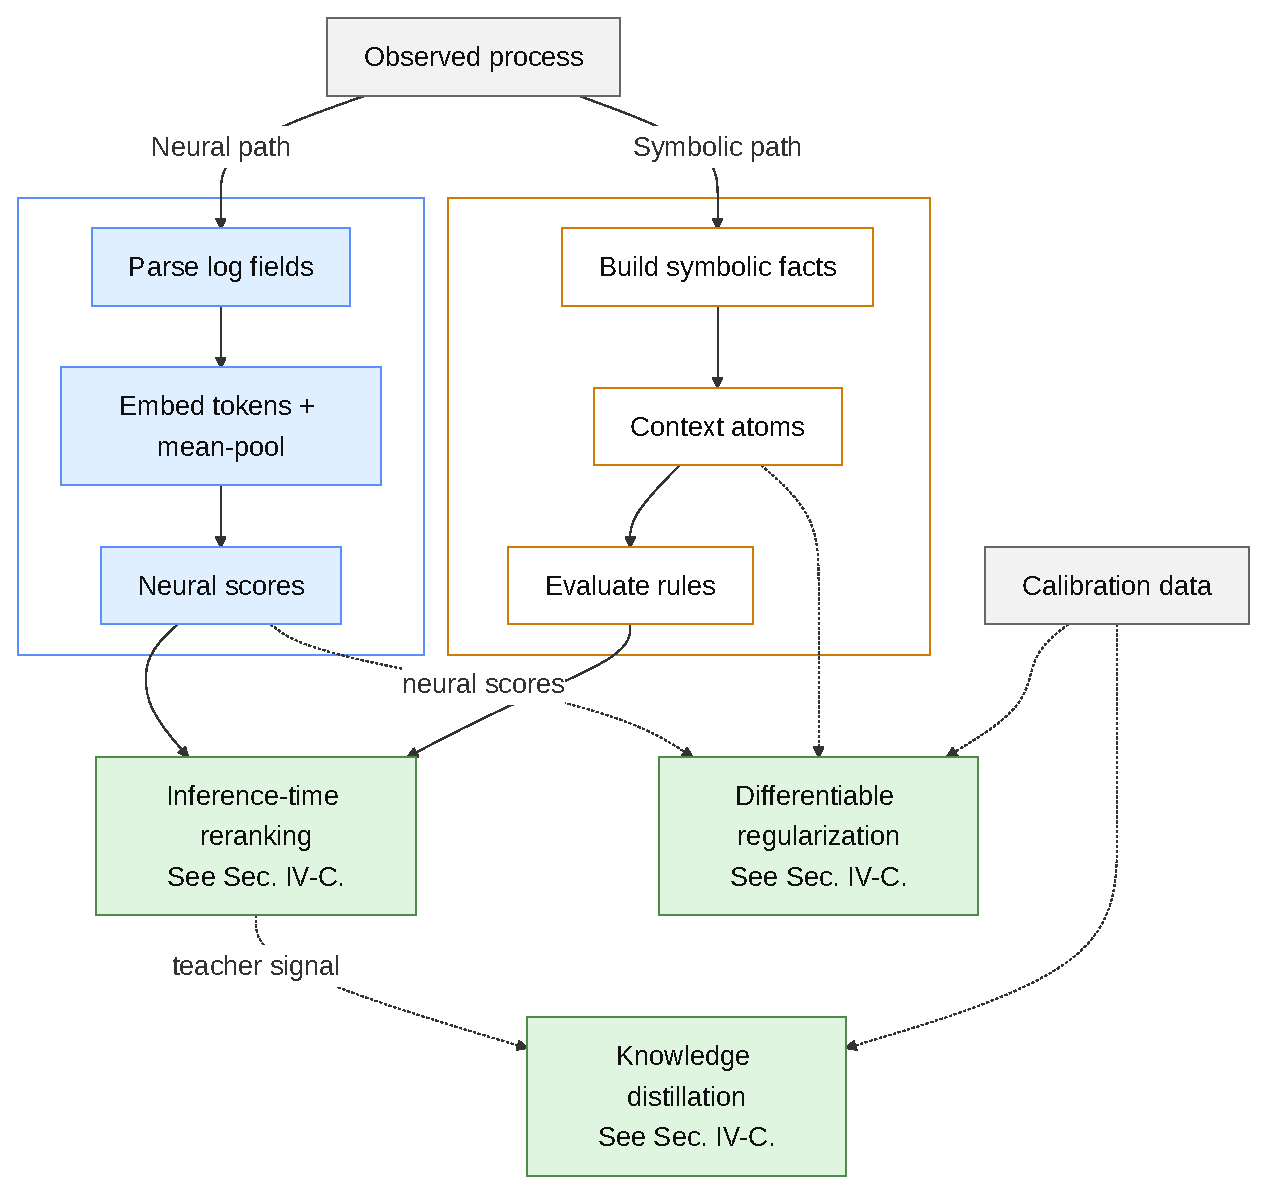
\includegraphics[width=.6\textwidth]{figures/postdoc/nesy/methodology_overview_cropped.pdf}%
\end{frame}

% 6. Results
{\setbeamercovered{transparent}
  \begin{frame}{Results}
    \centering
    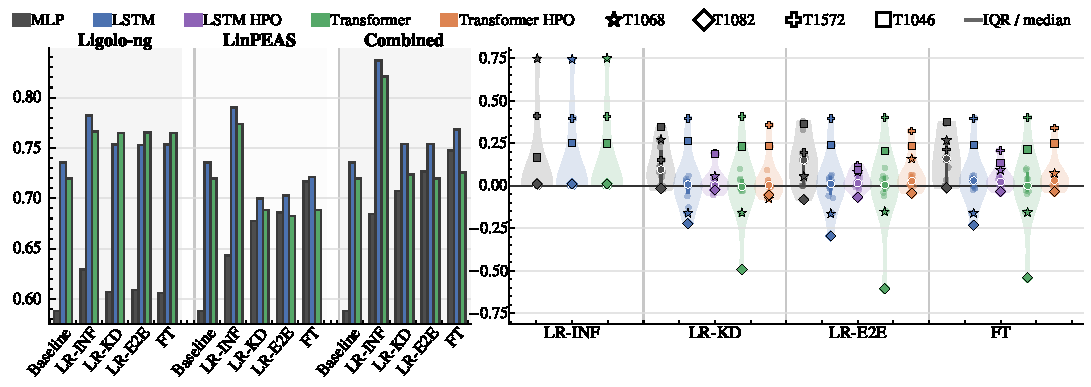
\includegraphics[width=0.9\textwidth]{figures/postdoc/nesy/results.pdf}
    \vspace{-0.8em}
    \begin{description}
        {\only<2>{\transparent{0.3}}%
      \item[Left:] Macro-F1 across backbones and integration methods: train-time outperforms inference-time, and can match LSTM/Transformer performance with a simple MLP backbone.}
        {\only<1>{\transparent{0.3}}%
      \item[Right:] Per-technique $\Delta$F1 versus the corresponding baseline: inference-time correction provide very consistent improvements across techniques.}
    \end{description}
  \end{frame}
}
% 7. Interests for Collab
% - inf time adaptation
% - auditability by interpretability
% - train smaller models and join With logic
\begin{frame}{Takeways}
  \begin{block}{Convincing proof of concept}
    Can effectively leverage \alert{domain knowledge} to improve performance, particularly with simple backbones.
  \end{block}

  \pause
  \begin{block}{Improved auditability}
    Symbolic rules provide \alert{interpretability} and can be used to audit model decisions.
  \end{block}

  \pause
  \begin{block}{Scaling problem}
    Automatic rule derivation is necessary to scale to more behaviors and scenarios.\pause{} \alert{Derive from provenance graphs?}
  \end{block}
\end{frame}
\section{Conclusion}

\begin{frame}{What about collaboration?}
  \stepcounter{beamerpauses}

  \begin{block}{Client-specific objectives}
    \textit{Learn globally, then adapt locally.}
    Facilitate collaboration while respecting \alert{client-specific constraints}.
  \end{block}

  \pause
  \begin{block}{Simpler learning objectives}
    \textit{Learn to recognize, not to reason.}
    Use logic reasoning for decision-making, with \alert{distributed representation learning} to provide confidential entity extraction across organizations.
  \end{block}

  %   \begin{itemize}[<+->]
  %     \item Problem: Logic programs might be too explicit to be shared (privacy concerns due to semantic richness)\dots \onslide<+->\emph{inapplicable to federated learning?}.
  %     \item Solution: use distributed representation learning to learn a shared embedding space for logic predicates, allowing for \alert{confidential} distributed reasoning.
  %   \end{itemize}
  % \end{block}

  \pause
  \bigskip\centering\rule{.4\textwidth}{.4pt}

  \medskip\Large \alert{Thank you!}

  \medskip\normalfont\ttfamily
  leo.lavaur@uni.lu | leolavaur.re
\end{frame}

% \begin{frame}{Where to?}
%   \centering
%   \includegraphics<+>[width=1.05\textwidth, trim={0 0 0 10pt}, clip]{figures/thesis/conclusion/beyond/12.pdf}%
%   \includegraphics<+->[width=1.05\textwidth, trim={0 0 0 10pt}, clip]{figures/project.drawio.pdf}%

%   \onslide<+->
%   \begin{tikzpicture}[remember picture,overlay]
%     \node[
%       anchor=north west,
%       yshift=-3em,
%       fill=white, fill opacity=0.85, text opacity=1,
%       text width=.7\textwidth,
%       align=left,
%       inner sep=.8em
%     ] at (current page.north west) {%
%       \small
%       \textbf{Collaborative \alert{neural-symbolic} reasoning}
%       \begin{itemize}
%         \item<4-> \alert{Simpler} (federated) learning objectives, which are more robust to heterogeneity and poisoning.
%         \item<5-> Use logic reasoning for \alert{interpretable} decision-making, with distributed representation learning to provide \alert{confidential} entity resolution across organizations.
%       \end{itemize}
%     };
%   \end{tikzpicture}
% \end{frame}

% \begin{frame}{Where to?}
%   \stepcounter{beamerpauses}
%   \begin{block}{\centering Collaborative \alert{neural-symbolic} reasoning}
%     \begin{itemize}
%       \item \alert{Simpler} (federated) learning objectives, which are more robust to heterogeneity and poisoning.
%       \item Use logic reasoning for \alert{interpretable} decision-making, with distributed representation learning to provide \alert{confidential} entity resolution across organizations.
%         %\item Pursue the development of \alert{independent} datasets.
%     \end{itemize}
%   \end{block}

% \end{frame}

\appendix

\begin{frame}[allowframebreaks]{References}
  \printbibliography[heading=none]
\end{frame}

\section*{Backup slides}

\begin{frame}
  \sectionpage
\end{frame}

\section{\S~Assessment Study}

\begin{frame}{Predictability}
  \begin{figure}
    \centering
    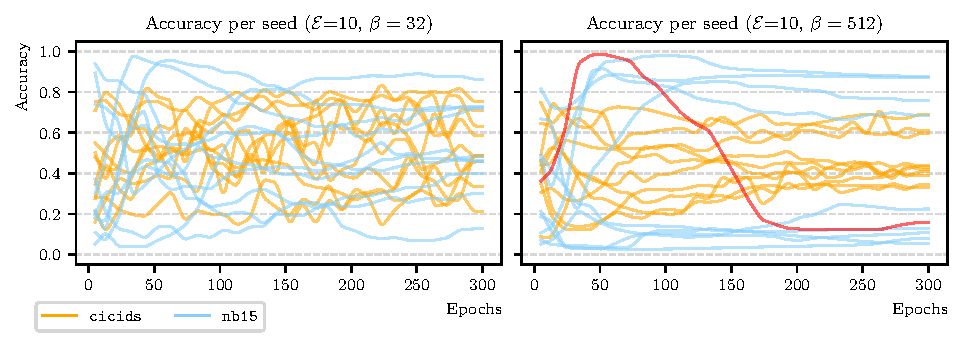
\includegraphics[width=0.8\textwidth]{figures/thesis/assessment/accuracy_per_seed.pdf}
    \caption{Accuracy of a FIDS under attack, across different random seeds.}
  \end{figure}
\end{frame}

\begin{frame}{Impact on attack propagation}
  \begin{figure}
    \centering
    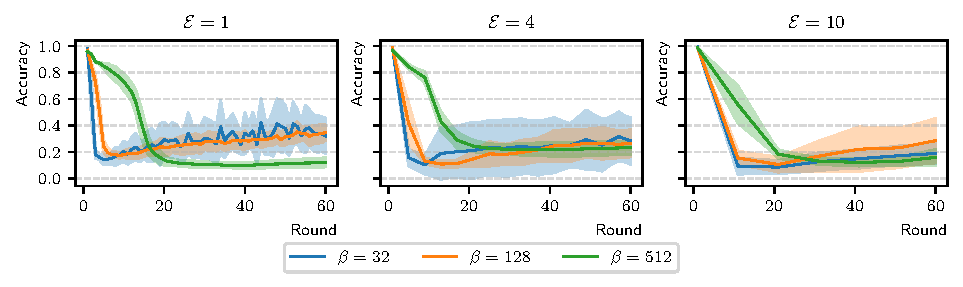
\includegraphics[width=0.8\textwidth]{figures/thesis/assessment/hyperparams-late-icdcs.pdf}
    \caption{Accuracy across rounds for different batch sizes.}
  \end{figure}
\end{frame}

\begin{frame}{Similarity-based Mitigation against Heterogeneity}

  \begin{columns}
    \begin{column}{.45\textwidth}
      \begin{itemize}[<+->]
        \item Known technique to detect poisoning attacks~\autocite{tolpegin_DataPoisoningAttacks_2020}.
        \item High heterogeneity makes it harder to detect attackers.
      \end{itemize}
    \end{column}

    \begin{column}{.55\textwidth}
      \begin{figure}
        \centering
        \foreach \i in {1,...,3}{%
          \includegraphics<\i>[width=\textwidth,trim={1cm 3cm 1cm 3cm},clip]{figures/thesis/assessment/similarity-untargeted-colluding-cicids-\i.pdf}%
        }
        \caption{PCA projection of the gradients in 2D (CICIDS).}
      \end{figure}
    \end{column}
  \end{columns}

  \footcite*{tolpegin_DataPoisoningAttacks_2020}

\end{frame}

\section{\S~Neural-symbolic AI}

\begin{frame}{IA neuro-symbolique\normalfont\normalsize~(\logic)}
  \begin{figure}
    \centering
    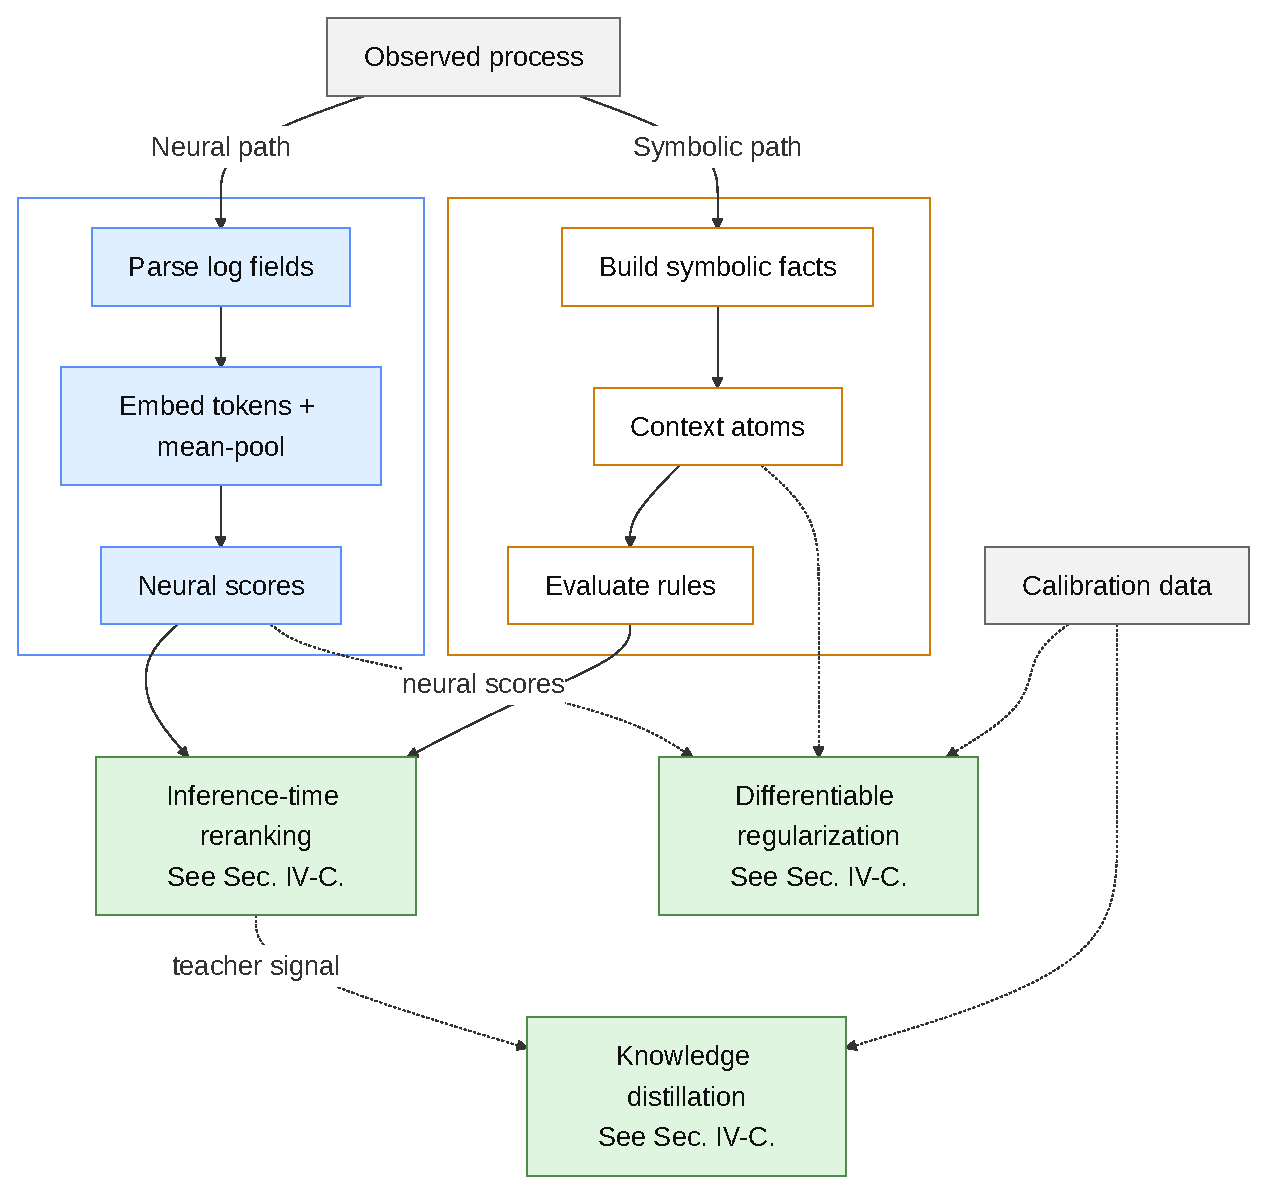
\includegraphics[width=0.5\textwidth]{figures/backup/nesy-detection.pdf}
    \captionof{figure}{Différentes intégrations neuro-symboliques.}
  \end{figure}
\end{frame}

\begin{frame}{IA neuro-symbolique\normalfont\normalsize~(\logic)}
  \centering
  \begin{table}
    \centering
    \caption{Fixing misclassification issues in CasinoLimit by adding contextual logic rules using Scallop.
    Macro-F1 on the targeted instances.}
    \small
    \begin{tabular}{llll}
      \toprule
      \textbf{Row} & \textbf{Ping (\texttt{ligolo-ng})} & \textbf{Grep (\texttt{linpeas.sh})} & \textbf{Combined} \\
      \midrule
      Baseline & 0.423277 & 0.423277 & 0.423277 \\
      Logic at inference & 0.455895 (+7.71\%) & 0.488943 (+15.51\%) & 0.521561 (+23.22\%) \\
      KL Distillation & 0.438017 (+3.48\%) & 0.533949 (+26.15\%) & 0.555552 (+31.25\%) \\
      Logic at training & 0.444519 (+5.02\%) & 0.560168 (+32.34\%) & 0.618868 (+46.21\%) \\
      %Relabelling & 0.444132 (+4.93\%) & 0.585468 (+38.32\%) & 0.697962 (+64.89\%) \\
      \bottomrule
    \end{tabular}
  \end{table}
\end{frame}

\begin{frame}{\texttt{Scallop}}
  \begin{figure}
    \centering
    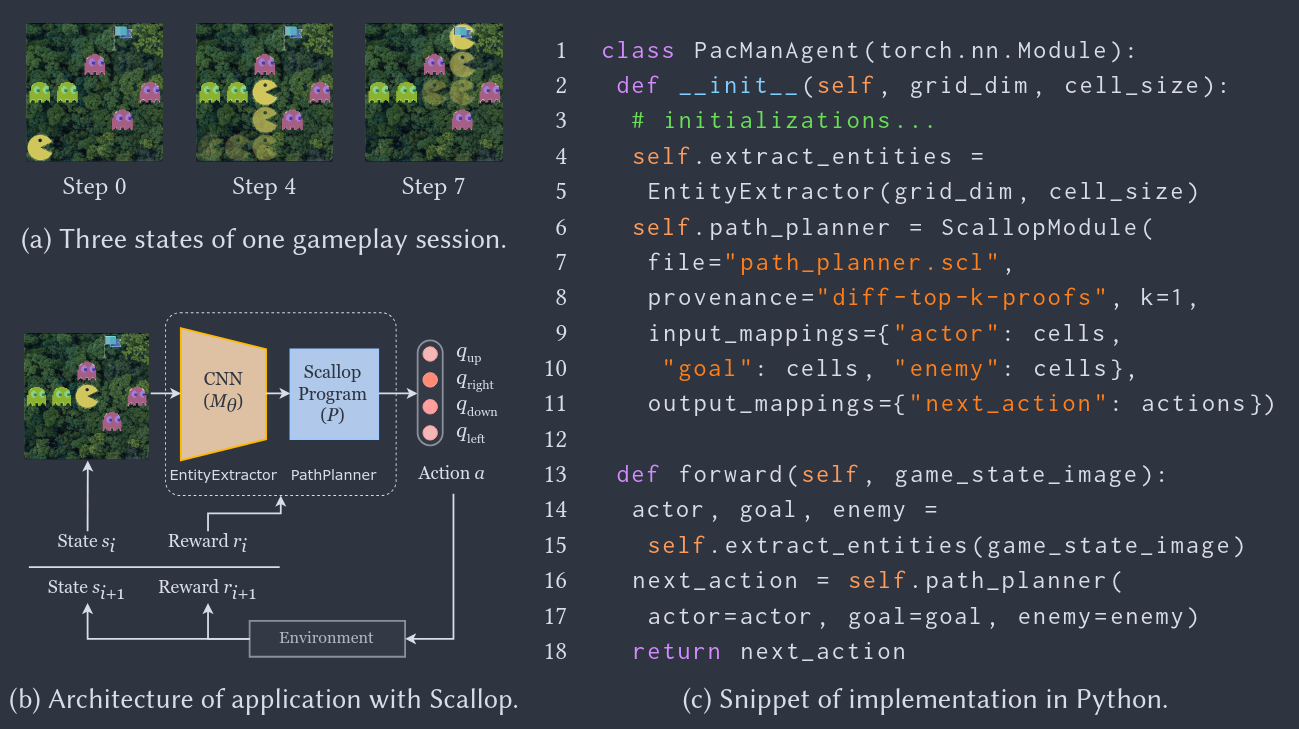
\includegraphics[width=0.75\textwidth]{figures/postdoc/scallop_appendix.png}
    \caption{Scallop~\footcite{huang_ScallopProbabilisticDeductive_2021}.}
  \end{figure}
\end{frame}

\begin{frame}{\texttt{DeepProbLog}}
  \begin{figure}
    \centering
    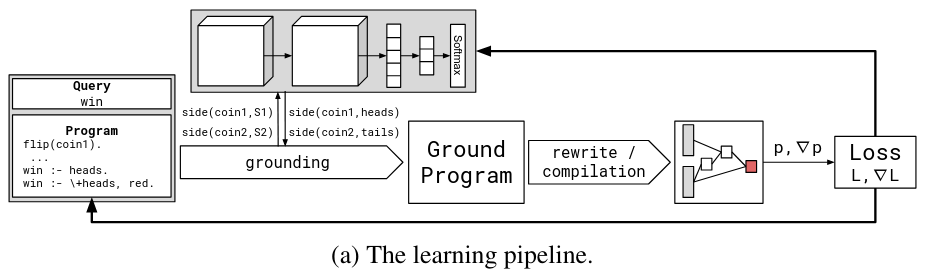
\includegraphics[width=0.8\textwidth]{figures/postdoc/deepproblog_appendix.png}
    \caption{DeepProbLog~\footcite{manhaeve_DeepProbLogNeuralProbabilistic_2018}.}
  \end{figure}
\end{frame}

\section{\S~\tt FedITN\_gen}

\input{sections/feditn/approach.tex}

\end{document}
